\chapter{Métodos y protocolos}\label{cap:metodos_critico}
\graphicspath{{figs/capitulo_metodos_critico/}}
\chapterquote{The method is the key to the door of knowledge. }{Galileo Galilei}



\section{Introducción}

%La imagen de calcio es un método poderoso para registrar la actividad de las poblaciones neuronales en muchas especies, pero la inferencia de los tiempos de disparo a partir de las señales de calcio es un problema desafiante. Comparamos varios enfoques utilizando varios conjuntos de datos con electrofisiología de referencia y encontramos que la simple deconvolución no negativa (NND) superó a todos los demás algoritmos en datos de prueba fuera de muestra.
%
%La imagen de calcio de dos fotones se puede utilizar para controlar la actividad de poblaciones de hasta 10,000 neuronas (Pachitariu et al., 2016; Stringer et al., 2018). Sin embargo, las señales de fluorescencia sensibles al calcio son una lectura indirecta de la actividad celular. Por lo tanto, se requerirán métodos de procesamiento de datos precisos y bien calibrados para aprovechar al máximo esta actividad (Vogelstein et al., 2010; Andilla y Hamprecht, 2014; Reynolds et al., 2015; Deneux et al., 2016; Theis et al., 2016; Friedrich et al., 2017; Jewell y Witten, 2017; Sebastian et al., 2017; Kazemipour et al., 2018). 
%
%
%
%Esta parte se muestran los algoritmos para inferir la serie de pulsos aproximadamente más probable de cada neurona, dadas las observaciones de fluorescencia.  



En este apartado, se presenta la metodología que se ha empleado para analizar tanto los datos experimentales del nematodo C. elegans como los resultados del modelo computacional. La precisión y robustez de los métodos desempeñan un papel crucial en la comprensión de las propiedades de criticidad neuronal y en la determinación de su emergencia en el sistema nervioso de C. elegans. La metodología abarca diversas técnicas de análisis de datos, métricas de criticidad, procesamiento de registros neuronales y ajuste de colas pesadas. Cada uno de estos pasos contribuye a una comprensión en profundidad de la dinámica neuronal a niveles microscópicos y macroscópicos.

En el \Cref{sec:inferencia_spikes}  se explicará el proceso detallado de procesamiento y análisis de los datos neuronales capturados durante la actividad espontánea del C. elegans. Esto incluye la identificación de eventos de disparo neuronal (spikes) y la extracción de información relevante de las grabaciones experimentales. Por otro lado en el \Cref{sec:clusteres} Se presentarán las métricas y técnicas empleadas para el análisis y la caracterización de los clústeres neuronales en el C. elegans. Esto incluye el uso del enfoque de componentes conexas y cómo se aplicó a los datos experimentales. Finalmente el \Cref{sec:leypotencia} Se describirá en detalle el procedimiento de ajuste de colas pesadas que se aplicó a los datos con el propósito de evaluar la distribución de eventos y la existencia de patrones relacionados con la criticidad. La comprensión detallada de cada etapa de la metodología es esencial para garantizar la confiabilidad y la significación de los resultados obtenidos. Estos métodos desempeñan un papel fundamental en la evaluación de las propiedades de criticidad neuronal, lo que contribuye significativamente a la comprensión de la dinámica del sistema nervioso en el C. elegans.




\section{Inferencia de spikes}\label{sec:inferencia_spikes}

El registro de la dinámica neuronal  simultanea de todo el sistema nervioso  de los distintos experimentos con  C elegans   se realizan mediante técnicas de  imágenes de señales de calcio  utilizando indicadores fluorescentes orgánicos o genéticamente codificados. Sin embargo, las señales de calcio son solo un proxy indirecto, a menudo no lineal y con filtro de paso bajo, de la variable de interés más fundamental, es decir, la serie de potenciales de acción (spikes) \cite{rupprecht_database_2021}. Un  problema clave en el análisis de los datos de imagen de calcio es la inferencia de los tiempos de spikes exactos a partir de la señal de calcio ruidosa, que tiene una dinámica más lenta que los spikes neuronales y se muestrean a una tasa de adquisición relativamente baja lo que hace que las transiciones inducidas por spikes individuales se solapen, a menudo sumándose de forma no lineal \cite{pnevmatikakis_bayesian_2013}. Además, las señales suelen estar contaminadas por  ruido, incluyendo las fluctuaciones de base similares a las respuestas reales.  Por lo tanto, la reconstrucción precisa de los spikes a partir de señales de calcio ruidosas es  una tarea computacional desafiante, debido a las limitaciones en la \gls{SNR} y la resolución temporal, los parámetros desconocidos y la intractabilidad analítica.  Para abordar este problema,  en este apartado se presentan los métodos  utilizados en este trabajo para inferir los tiempos de los potenciales de acción (spikes) a partir de las trazas de fluorescencia de los datos experimentales. Se busco que los algoritmos implementados   tuvieran  características tales como:  Poder analizar conjuntos de datos de imágenes de calcio a gran escala,   una reconstrucción de spikes sólida y precisa, una inferencia confiable sobre los parámetros y variables del método,  aplicable a una gran variedad de datos, computacionalmente eficiente y fácil de usar, en el sentido de que la intervención humana necesaria se limita al ajuste de unos pocos parámetros intuitivos.

\subsection{Algoritmos de deconvolución}


La concentración de calcio se observa como una serie de tiempo continua que aumenta bruscamente cuando la neurona se activa y posteriormente decae lentamente de manera exponencial con una constante de tiempo pequeña \cite{shibue_deconvolution_2020}. Si se producen múltiples spikes en un corto período de tiempo, la lenta disminución de la fluorescencia del calcio puede hacer que estos disparos se superpongan en el dominio temporal (ver \Cref{fig:dinamicacalcio}). Por  tanto los  algoritmos de deconvolución de spikes,  infieren una serie de spikes bajo la suposición de que la traza de fluorescencia representa una convolución aproximada de la serie de spikes subyacente con la respuesta de calcio de la célula. La deconvolución no negativa (NND) es un tipo de deconvolución que asume que las señales a desconvoluir son no negativas. Esto es razonable en el contexto de la imagen de calcio, ya que la fluorescencia de calcio es siempre positiva.  Una de las ventajas de los algoritmos NND es que son  muy robustos a las suposiciones sobre la forma supuesta de la respuesta del calcio a spikes únicos \cite{pachitariu_robustness_2018}. Se adopta  un enfoque completamente no supervisado para realizar la deconvolución donde en primer lugar se estima  un modelo paramétrico para la respuesta transitoria de la concentración de calcio que evocaría un solo spike.

 \begin{figure}[h!]
	\centering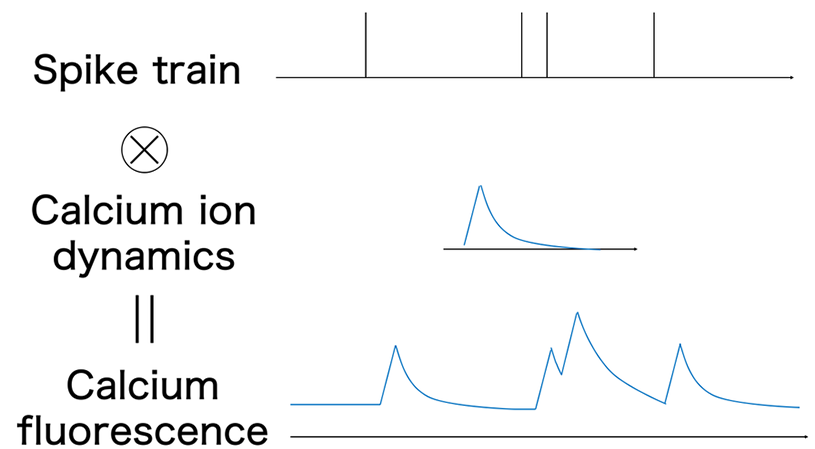
\includegraphics[width=\imsize]{dinamicacalcio.png}
	\caption[Superposición de la fluorescencia de calcio en el dominio temporal.]{Superposición de la fluorescencia de calcio en el dominio temporal. La fluorescencia de calcio observada  es la convolución de la dinámica de iones de calcio en un tren de spikes.  Si se producen dos picos en un tiempo corto en relación con la constante temporal de estas dinámicas, los aumentos de la concentración de iones de calcio debidos a estos picos se solaparán entre sí. (Figura adaptada de \protect\cite{shibue_deconvolution_2020})}\label{fig:dinamicacalcio}
\end{figure}




\subsubsection{Modelo autorregresivo de la dinámica del calcio}

La fluorescencia observada a menudo se considera como una comprensión ruidosa de la verdadera concentración de calcio subyacente.  Para modelar la actividad de una neurona, adoptamos un modelo popular en la literatura de neurociencia, donde la disminución de la fluorescencia se modela mediante un proceso autorregresivo y los spikes se modelan como saltos en correspondencia con los eventos de activación de la neurona.  Supongamos  que observamos la señal de fluorescencia durante $T$ intervalos de tiempo, y denotemos por $s(t)$ el número de spikes que la neurona disparó en el t-ésimo intervalo de tiempo, $t =1,\cdots, T$. Aproximamos las dinámicas de la concentración de calcio $c$ utilizando un proceso autorregresivo estable de orden $p$ ($AR(p)$) donde $p$ es un entero positivo pequeño,

\begin{equation}\label{eq:85}
	c(t)=\sum_{j=1}^{p}\gamma_jc\left(t-j\right)+s(t).
\end{equation}

La constante de tiempo $\gamma$ modela la tasa de tiempo de decaimiento más larga del indicador de calcio.  En palabras simples, el modelo $AR(p)$ asume que la concentración de calcio en el intervalo de tiempo actual $t$ depende de la concentración de calcio en los $p$ intervalos de tiempo anteriores. El valor de $p$ se elige típicamente entre 1 y 2, ya que valores más altos de $p$ pueden dar lugar a modelos que son demasiado complejos y difíciles de estimar \cite{pnevmatikakis_simultaneous_2016}.  Aunque  si se desea obtener  respuestas más estructuradas (por ejemplo, múltiples constantes de tiempo de decaimiento) también se pueden modelar los datos con valores más altos para el orden $p$. 

 La fluorescencia observada $y\in\mathbb{R}^T$ está relacionada con la concentración de calcio como:
 
 \begin{equation}\label{eq:86}
 	y(t)=\alpha c(t) + b  + \varepsilon(t), \quad \varepsilon(t) \sim \mathcal{N}(0,\sigma^2)
 \end{equation}
 

 
 El parámetro $\alpha$ absorbe todas las variables experimentales que influyen en la escala de la señal, incluido el número de sensores dentro de la célula, los fotones por ion calcio, la amplificación del sistema de formación de imágenes, etc. Del mismo modo, el offset $b$ absorbe, por ejemplo, la concentración de calcio de referencia de la célula, la fluorescencia de fondo del fluoróforo y el offset del sistema de formación de imágenes.   El ruido  $\varepsilon(t)$ en cada momento  se distribuye de forma  i.i.d según una distribución normal con media cero y varianza $\sigma^2$  \cite{vogelstein_fast_2010}. El objetivo de la deconvolución de calcio es extraer una estimación  de la actividad neuronal $\mathbf{s}$ del vector de observaciones $\mathbf{y}$. Esto conduce al siguiente problema de \gls{LASSO} no negativo para estimar la concentración de calcio:

\begin{equation}\label{eq:87}
	\underset{\hat{\mathbf{c}},\hat{\mathbf{s}}}{\text{minimize}} \quad  \frac{1}{2}\left\| \hat{\mathbf{c}}-\hat{\mathbf{y}}\right\|^2 +\lambda\cdot L(s) \quad \text{subject to}  \quad \hat{\mathbf{s}}\geq0
\end{equation}

donde $\left\|\cdot \right\|^2 $ es la norma euclidiana y $L(\mathbf{s})$ describe una función de penalización en los trenes de spikes inferidos.  El problema de optimización de la \cref{eq:87} se puede resolver utilizando solucionadores de programas convexos genéricos. Friedrich et al \cite{friedrich_fast_2017}   derivaron  un método mucho más rápido denominado Online Active Set method to Infer Spikes  (OASIS). El algoritmo se inspira en el algoritmo pool adjacent violators algorithm (PAVA). El algoritmo es  iterativo y  avanza a través de los datos y actualiza los valores estimados de la actividad neuronal. Cuando se detecta una violación de las restricciones, el algoritmo retrocede hasta el pico más reciente y vuelve a intentarlo. Este proceso continúa hasta que se alcanza el final de los datos.   OASIS ajusta los hiperparámetros $\lambda$ y $\gamma$ utilizando un método de validación cruzada. En la validación cruzada, el algoritmo  se ejecuta en un conjunto de datos de entrenamiento y se evalúa en un conjunto de datos de prueba. Los hiperparámetros que dan como resultado el mejor rendimiento en el conjunto de datos de prueba se seleccionan como los mejores hiperparámetros. Para una exposición más completa de este método como también una  interpretación en tiempo continuo del marco autorregresivo que conecta los coeficientes AR con algunas propiedades biofísicas de los indicadores de calcio se recomienda consultar los siguientes artículos \cite{pachitariu_robustness_2018,pnevmatikakis_simultaneous_2016,pnevmatikakis_bayesian_2013,friedrich_fast_2017}.


\subsubsection{Markov Chain Monte Carlo (MCMC)}\label{sec:MCMC}

Aunque el proceso de identificación de los parámetros  AR suele ser muy útil para estimar la respuesta transitoria que surgiría de un solo spike, es útil refinar estas estimaciones dadas las estimaciones iniciales de los tiempos de spike. Pnevmatikakis et al \cite{pnevmatikakis_simultaneous_2016} sugieren  que una extensión de los métodos bayesianos descritos en \cite{pnevmatikakis_bayesian_2013} proporcionan una estrategia eficaz. Este  enfoque bayesiano utiliza métodos de Montecarlo basados en cadenas de Markov  (\gls{MCMC}) para muestrear recursivamente los spikes y estimar la distribución posterior conjunta completa de todo el tren de spikes, condicionada a los datos de fluorescencia.  este enfoque goza de varias propiedades  deseables como la consistencia y estimaciones suaves de la posterior marginal del spike utilizando un esquema Rao-Blackwellizado.   

En la implementación que utilizamos  en este trabajo, el algoritmo utiliza un muestreador que muestrea directamente los tiempos de los spikes en tiempo continuo, dados los datos de calcio.  El espacio de estado corresponde al conjunto de tiempos de los spikes, y los movimientos transdimensionales cambian la dimensionalidad de este espacio de estado. En cada iteración, se muestrea el nuevo tiempo del i-ésimo pico $t_i$ dado la ubicación actual del resto de los picos y los hiperparámetros. Dado que el número de picos $K$ es en general desconocido, también se permiten  inserciones y eliminaciones de spikes en cada iteración.


\subsection{Algoritmos de aprendizaje profundo}

Recientemente, se ha afirmado que un nuevo enfoque para la detección de picos, basado en el aprendizaje supervisado profundo, supera a varios algoritmos de deconvolución existentes \cite{theis_benchmarking_2016}. Estos algoritmos aprenden a detectar spikes entrenándose con datos donde se conocen los tiempos de spike. Esto se hace alimentando al algoritmo con pares de señales de calcio y tiempos de spike que se miden electrofisiológicamente, y luego dejando que el algoritmo aprenda a asociar los dos. La principal ventaja de los algoritmos de aprendizaje supervisado es que potencialmente pueden lograr una mayor precisión que los algoritmos de deconvolución. Esto se debe a que pueden aprender a tener en cuenta factores que los algoritmos de deconvolución no pueden, como la forma de la señal de calcio y el ruido de los datos. Sin embargo, los algoritmos de aprendizaje supervisado también tienen algunas desventajas. Una es que requieren datos de \textquote{verdad fundamental}, que pueden ser difíciles y costosos de obtener. Otra es que es posible que no se generalicen bien a datos nuevos  realizados en condiciones diferentes a las de los datos de entrenamiento disponibles \cite{pachitariu_robustness_2018}.

Para superar estas limitaciones Rupprecht et al \cite{rupprecht_database_2021}  abordaron la cuestión de la generalización de forma sistemática. Para reunir una gran base de datos de la verdad fundamental, realizaron grabaciones intracelulares e imágenes de calcio de dos fotones utilizando diferentes indicadores de calcio y en diferentes regiones cerebrales de peces cebra y ratones. Esta base de datos se amplió con una cuidadosa selección de conjuntos de datos de la verdad fundamental disponibles públicamente. Utilizando esta gran base de datos, desarrollaron un método supervisado para la inferencia calibrada de spikes de datos de calcio utilizando redes profundas (\gls{CASCADE}). La red predeterminada consta de una red convolucional estándar con seis capas ocultas, incluidas tres capas convolucionales  (ver \Cref{fig:cascade}a). La entrada consiste en una ventana de 64 puntos temporales simétrica alrededor del punto temporal para el que se realiza la inferencia. Las tres capas convolucionales tienen tamaños de filtro relativamente grandes pero decrecientes (31, 19 y 5 puntos temporales), con un número creciente de características (20, 30 y 40 filtros por capa). Después de la segunda y la tercera capa, se insertan capas de pooling máximo. Una capa oculta densa final que consta de diez neuronas transmite el resultado a una sola neurona de salida. Aunque todas las neuronas en las capas ocultas se basan en ReLU, la neurona de salida se basa en una función de transferencia de identidad lineal. En total, el modelo consta de 18.541 parámetros entrenables.  




\begin{figure}[h!]
	\centering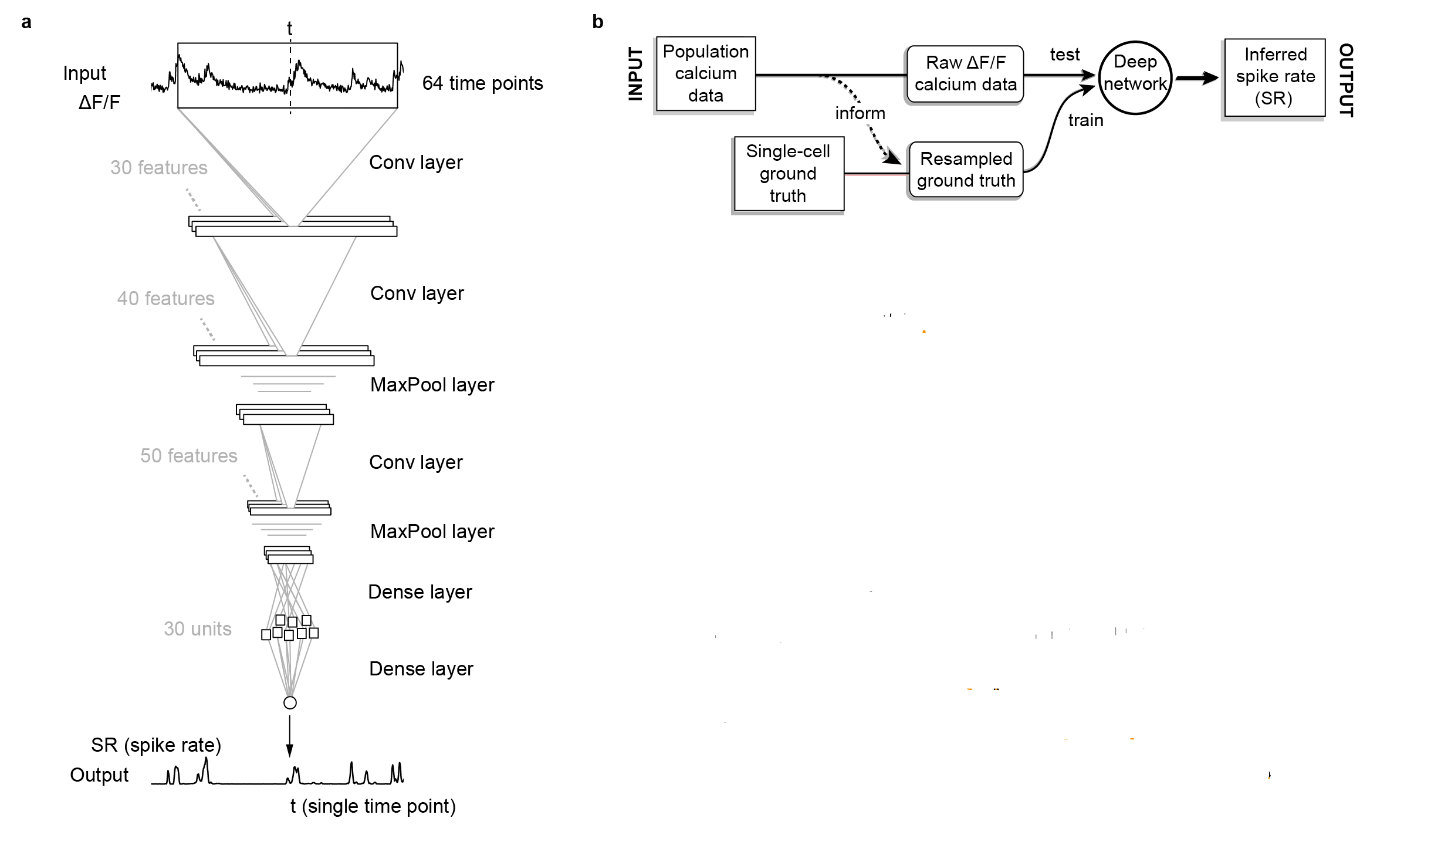
\includegraphics[width=\imsize]{cascade.png}
	\caption[El entrenamiento de una red profunda con la verdad fundamental ajustada al ruido mejora la inferencia de spikes.]{El entrenamiento de una red profunda con la verdad fundamental ajustada al ruido mejora la inferencia de spikes. (a) La red profunda por defecto consiste en una ventana de tiempo de entrada de 64 puntos de tiempo centrados alrededor del punto de tiempo de interés. A través de tres capas convolucionales, dos capas de agrupación y una pequeñ capa densa, la probabilidad de spike se extrae de la ventana de tiempo de entrada y se devuelve como un número único para cada punto de tiempo. (b), Se extraen las propiedades de los datos de población (velocidad de fotogramas y nivel de ruido; línea discontinua) y se utilizan para el remuestreo ajustado al ruido de los conjuntos de datos de la verdad fundamental existentes. La verdad fundamental remuestreada se utiliza para entrenar el algoritmo, resultando en una inferencia de spike calibrada de los datos de imagen de población (Figura adaptada de \protect\cite{rupprecht_database_2021})}\label{fig:cascade}
\end{figure}


CASCADE incluye métodos para volver a muestrear los conjuntos de datos originales de la verdad fundamental para que coincidan con su frecuencia de muestreo y nivel de ruido con un conjunto de datos específico de imágenes de calcio de interés. Este procedimiento permite entrenar algoritmos de aprendizaje automático bajo demanda en un amplio espectro de conjuntos de datos reales remuestreados, que coinciden con una amplia gama de condiciones experimentales (ver \Cref{fig:cascade}b). Por último, se probó sistemáticamente el rendimiento de CASCADE cuando se aplicó a datos no vistos. CASCADE fue robusto con respecto a cualquier elección de hiperparámetros y superó a los algoritmos existentes en las pruebas de referencia en todos los conjuntos de datos de verdad fundamental y niveles de ruido. El algoritmo CASCADE se puede utilizar directamente a través de una aplicación web basada en la nube y también está disponible, junto con los conjuntos de datos de verdad fundamental, como una caja de herramientas sencilla y fácil de usar basada en Python.

\subsection{Método de Kaplan para detectar picos neuronales}\label{sec:metodos_picos}

Finalmente,  el método de  detección de picos de Kaplan et al. \cite{kaplan_nested_2020}  también se utilizó para cuantificar los datos de actividad neuronal. Para todas las detecciones de picos, derivadas y no derivadas, adoptamos el siguiente enfoque:



\begin{enumerate}
	
	\item  A cada serie temporal $\Delta F/F_0$ de la actividad neuronal del experimento   se calcula sus derivadas temporales suavizadas con el método de Total-Variation Regularization  el cual es abordado en el \cref{C:ap1}. Para encontrar el parámetro de regularización  $\alpha$ optimo adoptamos un enfoque basado en principios y se utiliza un marco de optimización multiobjetivo para elegir los parámetros que minimizan una función de pérdida para equilibrar la fidelidad y la suavidad de la estimación de la derivada.  La función de pérdida para encontrar los parámetros óptimos esta dada por la \cref{eq:ap:1}, donde $\mathbf{y}$  son las series temporales, $\mathbf{\hat{\dot{x}}}$ es la estimación de la derivada,  $\text{trapz}(\cdot)$ es la integral numérica trapezoidal en tiempo discreto,  $\mu$	es la constante de integración desconocida,  $\gamma$ es un hiperparámetro, y  $TV$  es la variación total dada por la \cref{eq:ap:2}.  Para encontrar el parámetro $\gamma$ que minimiza a la \cref{eq:ap:1}   Van Breugel et al \cite{van_breugel_numerical_2020} propusieron que la mejor elección de $\gamma$ depende del contenido frecuencial de los datos. En resumen, la elección óptima de $\gamma$ , suponiendo que se valora tanto un RMSE bajo como una baja correlación de errores, puede hallarse según la siguiente relación: 
	
	
	\begin{equation}\label{eq:84}
		\log (\gamma) = -1.6\log (f) -0.71\log (dt) -5.1.
	\end{equation}
	
	A partir de los espectros de potencia que serán calculados mediante la función  de Scipy \textbf{scipy.signal.periodogram}, seleccionamos una frecuencia $f$ correspondiente a aquella en la que la potencia empieza a disminuir y el ruido del espectro aumenta. Aunque un tanto arbitrario, este enfoque (junto con la \cref{eq:84}) nos permite utilizar una herramienta estándar de procesamiento de señales para determinar rápidamente una elección de $\gamma$. Para facilitar la aplicación a nuestros datos del anterior marco de optimización utilizamos la biblioteca de Python de código abierto, \textbf{pynumdiff} \footnote{La documentación se puede encontrar en  el siguiente enlace \url{https://github.com/florisvb/PyNumDiff}}.  El  objetivo de este paquete es desarrollar un enfoque general para elegir metódicamente parámetros que equilibren la necesidad de minimizar tanto el error como el sesgo. 
	
	\item Para todas las detecciones de los picos, tanto en las  derivadas como en los datos de las series temporales, adoptamos el siguiente enfoque
	\begin{itemize}
		\item Mediante la función de  de Scipy   \textbf{scipy.signal.find\_peaks} detectamos máximos y mínimos locales en cada serie temporal: los picos máximos se encontraron como valores máximos que iban precedidos y seguidos de valores mínimos separados del máximo por una diferencia de amplitud de al menos delta, un parámetro clave.  La detección de picos implica un compromiso entre falsos positivos y falsos negativos; el parámetro delta determina lo liberal (más falsos positivos) o conservadora (más falsos negativos) que es la detección de picos. Se ha desarrollado un método sencillo para determinar automáticamente un valor de delta casi óptimo (es decir, que minimice tanto los falsos positivos como los falsos negativos). Para cada serie temporal   se realiza lo siguiente,  
		
		\begin{enumerate}[label=(\roman*)]
			\item realizamos la detección de picos con un amplio rango de deltas  que va desde demasiado liberal (muchos falsos positivos, debido a la detección de ruido) a demasiado conservador (muchos falsos negativos, algunos picos de gran amplitud no serán detectados). 
			\item graficamos el número de picos detectados en función de delta. La forma de esta curva varía en función de la serie temporal, pero a menudo se asemeja a una función lineal definida a trozos  de dos partes. En valores bajos de delta, la pendiente es alta: el número de picos detectados  está dominado por falsos positivos debido al ruido y, en este caso, pequeños aumentos de delta provocan grandes disminuciones del número de picos detectados. En valores altos de delta, la pendiente es baja: los picos detectados  son sólo reales (es decir, de gran amplitud) y, en este caso, pequeños aumentos de delta suelen dar lugar a poco o ningún cambio en el número de picos detectados. Por lo tanto, la pendiente de la curva en valores delta altos está mucho más cerca de 0 que en valores delta bajos.  En el caso ideal, el punto de cambio entre estas dos líneas es claro, dando un valor delta óptimo en el que se minimiza el número tanto de falsos positivos como de falsos negativos. 
			\item Suavizamos la curva de picos utilizando un filtro de Savitzky-Golay utilizando la función de Scipy \textbf{scipy.signal.savgol\_filter} . La principal ventaja de esta aproximación es que tiende a preservar características de la distribución inicial tales como los máximos y mínimos relativos, así como el ancho de los picos, que normalmente desaparecen con otras técnicas de promediado (como la media desplazada).
			\item Para detectar el punto de cambio utilizamos uno de los algoritmos disponibles para la detección  de múltiples puntos de cambio en series temporales multivariadas revisados por  Truong et al \cite{truong_selective_2020}.   Truong et al adoptaron una estrategia metodológica general. Los algoritmos de detección considerados se caracterizan por tres elementos: una función de coste, un método de búsqueda y una restricción sobre el número de cambios. Cada uno de estos elementos se describe, revisa y discute por separado en el articulo original  \cite{truong_selective_2020}. Las implementaciones de los principales algoritmos descritos en este artículo se proporcionan dentro de un paquete de Python llamado \textbf{ruptures}\footnote{La documentación de la librería se encuentra en: \url{https://centre-borelli.github.io/ruptures-docs/}}  el cual utilizamos en nuestros datos. Utilizamos el algoritmo que produce  el índice de la curva en la que tanto la media como la pendiente cambian más abruptamente.
		\end{enumerate}
		
		\item Para la detección de picos en derivadas, se realizaron dos pasos adicionales:
		\begin{enumerate}[label=(\roman*)]
			\item se excluyeron los picos con amplitudes inferiores a 0, ya que se trata de cambios en la pendiente de una caída y no de subidas; 
			\item el segundo de dos máximos posteriores sólo se incluyó si el mínimo intermedio caía por debajo de 0. Si el mínimo intermedio no caía por debajo de 0, los dos picos correspondían a cambios en la pendiente y no a picos de calcio individuales, por lo que se excluyó el segundo pico.
		\end{enumerate}
		
	\end{itemize}
\end{enumerate}


\section{Clústeres de la dinámica neuronal}\label{sec:clusteres}

Definimos los clústeres como conjuntos máximos de neuronas que comparten el mismo tipo de actividad (en el modelo de Haimovici estados activos) conectados siguiendo la matriz de adyacencia. El tamaño del clúster es el número total de neuronas participantes. Entre todos los tamaños de clústeres, nos centramos en los dos mas grandes, $S_1$ y $S_2$ como también el tamaño promedio de los clústeres $\chi$ que son parámetros de orden estándar en la teoría de la percolaciones. Medimos los tamaños promediados durante el tiempo de simulación $t_{sim}$ comenzando desde un tiempo transitorio  $t_{tran}$:

\begin{equation}\label{eq:80}
	\bar{s}_i=\frac{1}{t_{sim}-t_{tran}}\sum_{t=t_{tran}}^{t_{sim}}s_i(t), \quad i=1,2
\end{equation}
donde $s_i(t)$  es el tamaño del i-ésimo  clúster más grande encontrado en el tiempo $t$.   Con las \cref{eq:80,eq:15}  se puede calcular el tamaño promedio de clústeres $\chi$.  La distribución del tamaño de los clústeres depende crucialmente de $T$ y se utiliza para construir dos indicadores de criticidad bien establecidos: (a) un cambio abrupto en el tamaño promedio temporal de $S_1$
y (b) un pico en el tamaño promediado en el tiempo de $S_2$ y $\chi$; ambos ocurren cerca del umbral crítico $T_C$. 

\subsection{ Componentes conexas }

Para calcular los clústeres   tanto de la dinámica neuronal de los experimentos como del modelo computacional utilizamos un algoritmo que calcula las  componentes conexas de los estados neuronales de la dinámica del sistema.   Un grafo no dirigido es conexo si existe un camino entre cualquier par de vértices. El grafo de la Figura 3.6 no es conexo porque, por ejemplo, no hay camino de A a K. Sin embargo, tiene tres regiones conexas disjuntas, correspondientes a los siguientes conjuntos de vértices:

\begin{equation*}
	\left\{A,B,E,I,J\right\} \quad \left\{ C,D,G,H,K,L\right\} \quad \left\{ F\right\}
\end{equation*}

Estas regiones se denominan componentes conexas: cada una de ellas es un subgrafo internamente conexo pero que no tiene aristas hacia los restantes vértices.   Mas formalmente  una componente conexa de un grafo no dirigido $G = (V, E)$ es un conjunto máximo de vértices $S \subset V$ tales que para cada $u \in  S$ y $v \in  S$, existe un camino en $G$ desde el vértice $u$ hasta el vértice $v$ \cite{componetes1}.

\begin{definitionT}[Componente conexa]
	Sea $u \sim v$ si y solo si $G$ tiene un camino desde el vértice $u$ hasta el vértice $v$. Esta es una relación de equivalencia (es simétrica, reflexiva y transitiva). Entonces, una componente conexa de $G$ es una clase de equivalencia de esta relación $\sim$. Recuérdese que la clase de equivalencia de un vértice $u$ sobre una relación $\sim$ es el conjunto de todos los vértices $v$ tales que $u \sim  v$.
\end{definitionT}

Para un grafo dirigido, hay dos tipos de componentes: 

\subsubsection{Componente fuertemente conexa}


una componente fuertemente conexa tiene una ruta dirigida entre dos nodos, 
\begin{definitionT}[Componentes fuertemente conexas (SCC)]
	Una componente fuertemente conexa en un grafo dirigido $G = (V, E)$ es un conjunto máximo de vértices $S \subset V$ tal que cada vértice  $v \in S$ tiene un camino a cada otro vértice $u\in S$. Esto es lo mismo que la definición usando clases de equivalencia para grafos no dirigidos, excepto que ahora $u \sim v$  si y solo si hay un camino de $u$ a $v$ y un camino de $v$ a $u$.
\end{definitionT}

\subsubsection{Componentes débilmente conexas}
Una componente débilmente conexa ignora la dirección y solo requiere que exista una ruta entre dos nodos,

\begin{definitionT}[Componentes débilmente conexas (WCC)]\label{WCC}
	Sea $G = (V, E)$ un grafo dirigido, y sea $G^\prime$ el grafo no dirigido que se forma sustituyendo cada arista dirigida de $G$ por una arista no dirigida. Entonces las componentes débilmente conexas de $G$ son exactamente las componentes conexas de $G^\prime$.
\end{definitionT}

Para grafos dirigidos, los algoritmos usuales para calcular las Componentes fuertemente conexas (SCC)  son el algoritmo de Kosaraju, algoritmo de componentes fuertemente conectados de Tarjan, algoritmo de componentes fuertes basado en el camino. 

\subsection{Algoritmo de clústeres neuronales }\label{sec:alg_cluster}

Tanto en los experimentos como en el modelo computacional utilizamos un algoritmo de  componentes débilmente conexas para calcular los clústeres en cada paso de tiempo. El grafo en  el cual  se encontraron los clústeres de neuronas sincronizadas es el conectoma del C. elegans. Este grafo no se mantiene estático si no que evoluciona dinámicamente    como consecuencia de la dinámica neuronal del sistema. En cada paso de tiempo las componentes conexas del  grafo  (ver por ejemplo la figura)   cambian de forma dinámica ya que  que se forman o se pierden conexiones entre nodos  como consecuencia de que el estado de cada uno de estos evoluciona siguiendo las reglas de transición del sistema y solo las conexiones entre nodos en el estado excitado forman parte de estas componentes.   El \cref{alg:CC}   calcula los clústeres de neuronas sincronizadas en cada paso de tiempo.  Primero el grafo dirigido del conectoma $G$ se convierte en su equivalente no dirigido $G^\prime$ (\cref{WCC}). En cada paso de tiempo  se eliminan los  vértices que no están en el estado excitado ( y por ende las conexiones que estos puedan tener con otros nodos) esto crea un grafo $\tilde{G}$ no conexo en el cual se  se buscaran sus componentes conexas.    Para encontrar una componente conexa de este grafo $\tilde{G}$, podemos elegir un nodo y comenzar a hacer una búsqueda (\gls{BFS}, \gls{DFS} o  Unión-Buscar) de ese nodo \cite{dasgupta_algorithms_2006}. Todos los nodos que podemos alcanzar desde ese nodo componen una sola componente conexa. Para encontrar todas las componentes conexas, entonces solo necesitamos pasar por cada nodo, encontrando sus componentes conexas una a la vez buscando en el grafo. Sin embargo, no se necesita buscar en un nodo $V$ si ya se ha encontrado que es parte de una componente conexa anterior. Por lo tanto, si se realiza  un seguimiento de los nodos que ya se han encontrado, solo se debe realizar   un \gls{DFS} (o \gls{BFS}) para cada componente conexa.   El algoritmo también mantiene un vector $cc(v)$ para cada nodo $V$, para recordar qué componente conexa lo contiene.  Las búsquedas en este algoritmo toman tiempo total $\mathcal{O}\left(\left|V\right| + \left|E\right| \right)$, porque cada llamada \gls{BFS} o \gls{DFS} lleva tiempo lineal en el número de enlaces y nodos para su componente, y cada componente solo se busca una vez, por lo que todas las búsquedas tomarán tiempo lineal en el número total de enlaces y nodos.  

\begin{algorithm}{Componentes débilmente conexas}{CC}
	\textbf{Entradas:}  El grafo dirigido del conectoma  $G = (V, E)$ en representación de lista de adyacencia, siendo $V = \{1, 2, 3, \cdots , N\}$ las neuronas y $\mathbf{s}=\{s_1,s_2,\cdots,s_N\}\quad s_i\in\mathcal{E}=\left\{Q,E,R\right\}$ los estados de cada una de ellas.
	
	\textbf{Salida:}   el vector $cc[v]$ que asigna a cada nodo $v$ un número entero  que identifica el componente conectado al que pertenece. Para todo $u, v \in  V$, $cc(u) = cc(v)$ si y sólo si $u, v$ están en la misma componente conexa.
	
	\begin{pseudo}[indent-mark]
		\ct{Convierte el grafo dirigido $G(V,E)$ en su equivalente no dirigido $G^\prime (V,E) $} \\
		$G^\prime (V,E) $ =   \pr{To\_undirected}($G(V,E)$)   \\
		\kw{for} \tn{each}  $v\in V$ \kw{do}  \\+
		\kw{if} $s[v] \== E$ \kw{then}                           \\+ 
		$\tilde{V}  \leftarrow v$ \\--
		marcar todos los vértices como inexplorados \\
		$numCC \coloneqq 0$ \\
		\kw{for} \tn{each}  $\tilde{v}\in \tilde{V}$ \kw{do}  \ct{prueba todos los vértices}  \\+		
		\kw{if}  $\tilde{v}$ is  unexplored  \kw{then}  \ct{evitar la redundancia} \\+		
		$numCC \coloneqq numCC + 1$ \ct{nuevo componente} \\
		\ct{Utilizamos BFS} \\
		$Q \coloneqq$ una estructura de datos de cola, inicializada con $\tilde{v}$\\
		\kw{while} $Q$ is not empty \kw{do} \\+
		quitar el vértice de la parte inicial de $Q$\\
		$cc(\tilde{v}) := numCC$\\
		\kw{for} each ($\tilde{v}$, w) in la lista de adyacencia de $\tilde{v}$ \kw{do} \\+
		\kw{if}  $w$ is unexplored \kw{then} \\+
		marcar $w$ como explorado \\
		añadir $w$ al final de Q \\
	\end{pseudo}
\end{algorithm}



\subsection{Medición de la densidad de números de clústeres}\label{sec:medicion_clusteres}

Como se discutió en el apartado anterior, tanto  en la simulaciones  y en los datos experimentales  el sistema se caracterizá por una amplia distribución de clústeres, es decir, regiones de nodos conectados. Los clústeres tienen diferente formas y tamaños. Si aumentamos $p$ para acercarnos a $p_c$,  los clústeres aumentan de tamaño hasta alcanzar el tamaño del sistema. Donde el tamaño se refiere al número de $nodos$ en un clúster.  En la teoría de la percolación, caracterizamos los tamaños de los clústeres haciendo una pregunta concreta: Si apuntamos a un nodo (aleatorio) en la red, ¿cuál es la probabilidad de que este nodo pertenezca a un clúster de tamaño $s$?,  esta probabilidad esta dada por $sn(s,p)$, donde $n(s,p)$ es la densidad del número de clústeres  que es la probabilidad de que un nodo sea un nodo específico en un clúster de tamaño $s$.\cite{percolacion_python}.

Para estudiar  la distribución de clústeres numéricamente  introducimos un histograma de tamaños de clústeres. Escribimos $N_s$ como el número de clústeres de tamaño $s$.  ¿Cómo podemos ahora estimar $sn(s, p)$, la probabilidad de que un nodo dado sea parte de un clúster de tamaño $s$, a partir de $N_s$? La probabilidad de que un nodo pertenezca a un clúster de tamaño $s$ puede estimarse dividiendo el número de nodos que pertenecen a un clúster de tamaño $s$ por el número total de nodos. El número de nodos que pertenecen a un clúster de tamaño $s$ es $sN_s$, y el número total de nodos es $L^d$, donde $L$ es el tamaño del sistema y $d$ es la dimensionalidad. Para producir buenas estimaciones estadísticas para $n(s, p)$ debemos muestrear a partir de muchas realizaciones aleatorias del sistema. Si muestreamos a partir de $M$ realizaciones, y luego medimos el número total de clústeres de tamaño $s$, $N_s(M)$, sumado sobre todas las realizaciones, estimamos la densidad de números de clúster a partir de: 

\begin{equation}\label{eq:88}
\overline{n(s,p;L)}=\frac{N_s(M)}{L^d\cdot M}.
\end{equation}

donde usamos una barra para mostrar que esta es una cantidad estimada y no la probabilidad real. Se debe tener  en cuenta que todas las simulaciones son para $L$ finito, por lo que esperamos desviaciones debido a $L$, así como aleatoriedad debido al número finito de muestras. Sin embargo, esperamos que el $\overline{n(s, p; L)}$ estimado se acerque al $n(s, p)$ subyacente a medida que $M$ y $L$ se acerquen al infinito.



 \section{Ajuste de distribuciones de cola pesada}\label{sec:leypotencia}




En este apartado abordamos un tema recurrente en la literatura científica, la cuestión de cómo reconocer una ley de potencia en datos empíricos. En la práctica, rara vez o nunca podemos estar seguros de que una cantidad observada se extraiga de una distribución de ley de potencia. Lo máximo que podemos decir es que nuestras observaciones son consistentes con la hipótesis de que $x$ se extrae de una distribución  con forma de ley de potencia \cite{clauset_power-law_2009}. Otra de las cuestiones pendientes en la literatura es el ajuste preciso de distribuciones de ley de potencia discretas doblemente truncadas (es decir, distribuciones con un límite mínimo y máximo).   Esta cuestión es significativa porque la gran mayoría de los datos reales potencialmente de ley de potencia están doblemente truncados \cite{marshall_analysis_2016}. El límite máximo suele estar causado por efectos de tamaño finito. En nuestros datos experimentales y del modelo de criticidad  hay límites prácticos como el  máximo numero de neuronas que pueden registrarse simultáneamente y  el número máximo de neuronas en el cerebro del C. elegans.


Descuidar la existencia de estos límites máximo en los datos  puede conducir a resultados inexactos, incluso cuando los datos son verdaderamente descritos por una  ley de potencia. Esto se debe a que las distribuciones de ley de potencia doblemente truncadas no producen funciones de distribución acumuladas (CDFs) de ley de potencia y  por ende muchos  de los métodos en la literatura convencional (ver por ejemplo \cite{clauset_power-law_2009})  basados en esta distribución podrían producir  resultados inexactos. En esta sección describimos dos nuevos métodos que abordan estas preocupaciones y son más precisos para ajustar datos de ley de potencia doblemente truncados.  El primer método que trataremos es una extensión  de  las técnicas de MLE (estimación de máxima verosimilitud) previamente utilizadas (\cite{clauset_power-law_2009}).  Mientras que el segundo  propone una estrategia de promedio para los mínimos cuadrados ordinarios denominada LSavg.



\subsection{Primer método}

Para una ley de potencia discreta truncada, la función de masa de probabilidad se da mediante la ecuación


\begin{equation}\label{eq:90}
	p(x)=A\left(\alpha, x_{min}, x_{max}\right)\left(\frac{1}{x}\right)^\alpha.
\end{equation}

$A$  es una constante de normalización, $\left\{x\in\mathbb{Z}: x_{min}\leq x \leq x_{max} \right\}$, $\left\{\alpha\in\mathbb{R}:\alpha>1\right\}$, $x_{min}$ es el valor mínimo de $x$ y $x_{max}$ es el valor máximo. El valor de $A$ se puede encontrar normalizando la función de masa de probabilidad

\begin{equation}
	A(\alpha,x_{min},x_{max})=\frac{1}{\sum_{x=x_{min}}^{x_{max}}\left(\frac{1}{x_i}\right)^{\alpha}}.
\end{equation} 

La función de verosimilitud $L(\alpha)$ para todas las $N$ mediciones individuales $x_i$ se da mediante 

\begin{equation}
	L(\alpha)=\prod_{i=1}^{N}p(x_i)=A(\alpha,x_{min},x_{max})^N\prod_{i=1}^{N}\left(\frac{1}{x_i}\right)^{\alpha}.
\end{equation}
Entonces, la verosimilitud logarítmica se da mediante 

\begin{equation}\label{eq:91}
	l(\alpha)=-\log\left(\sum_{x=x_{min}}^{x_{max}}\left(\frac{1}{x}\right)^\alpha\right)-\frac{\alpha}{N}\sum_{i=1}^{N}\log(x_i).
\end{equation}

La primera expresión de la \Cref{eq:91} es monótonamente creciente en $\alpha$, mientras que el segundo término es linealmente decreciente en $\alpha$. Por lo tanto, habrá un valor máximo único para $l(\alpha)$.  Se utiliza un algoritmo (\Cref{alg:ABR}) de búsqueda de red para estimar el exponente de la ley de potencia $\alpha_{fit}$ que maximiza $l(\alpha)$.

\begin{algorithm}{Búsqueda de red}{ABR}
	
	\begin{pseudo}[indent-mark]
	Comenzar con un intervalo inicial para $\alpha$.\\
	Calcular $l(\alpha)$ para cada valor de $\alpha$ en el intervalo.\\
	Seleccionar el valor de $\alpha$ que maximiza $l(\alpha)$.\\
	Reducir el intervalo para $\alpha$ en función del valor seleccionado en el paso 3.\\
	Repetir los pasos 2 a 4 hasta que se alcance una precisión deseada.
	\end{pseudo}
\end{algorithm}


\subsubsection{ Prueba de la hipótesis de la ley de potencia}\label{sec:ajusteybondad}


Dado que es posible ajustar una distribución de ley de potencia a cualquier conjunto de datos, es apropiado probar si los datos observados realmente siguen una ley de potencia.  Por lo tanto, se utiliza  el siguiente procedimiento para cuantificar ajustes aceptables. 


\begin{procedimiento}[Prueba de la hipótesis de la ley de potencia]
\phantom{text}
\begin{enumerate}
\item Utilizar un modelo de ley de potencia para producir conjuntos de datos sobre el rango de ajuste.
\item Comparar las estadísticas de la prueba de Kolmogorov-Smirnov (KS) entre los datos reales y el ajuste frente a los datos modelo y el ajuste.
\item Si los datos reales producían una estadística KS que era menor que la estadística KS encontrada para al menos el 20\% de los modelos de ley de potencia (es decir, $p \geq pthresh = 0.2$), se aceptan los datos como ajustados por la ley de potencia truncada.
\item Si lo contrario era cierto, se rechaza la hipótesis de que los datos se ajustan mediante una ley de potencia truncada.
\end{enumerate}
\end{procedimiento}

\subsection{Segundo método}

La estimación por mínimos cuadrados ordinarios (LSE) se ha demostrado que es el mejor estimador lineal insesgado con mínima varianza entre la clase de estimadores lineales insesgados según el teorema de Gauss-Markov.  Zhong et al.  \cite{zhong_is_2022} propusieron una estrategia de promedio para los LSE ordinarios denominada LSavg para estimar los parámetros de los modelos de ley de potencia. La idea que subyace a la estrategia de promedio es que si un conjunto de puntos de datos sigue perfectamente una distribución de ley de potencia, entonces el uso de cualquier subconjunto de dos o más puntos de datos puede encontrar la pendiente óptima de la línea en el sistema doblemente logarítmico, y todas estas pendientes y su media aritmética son iguales. 
\section{Metodología}

Para un conjunto de puntos de datos, si siguen una distribución de ley de potencia, entonces pueden caracterizarse por la ecuación

\begin{equation}\label{eq:92}
	p(x)=K\cdot x^{-\alpha},
\end{equation}
donde $\alpha$ es el exponente de escala y $K$ es una constante. Sacando $\log$ a ambos lados de la \Cref{eq:92} encontramos 

\begin{equation}\label{eq:93}
	s=\alpha\cdot t+ c,
\end{equation}

donde $s=-\log p(x)$, $t=\log x$, y $c=-\log K$. Dada una serie de puntos de datos $\left\{(t_i,s_i)\right\}, 1 \leq i\leq N$ que siguen una línea como la  \Cref{eq:93}, se utiliza  LSE para encontrar el valor óptimo de $\alpha$ resolviendo:

\begin{equation}
	\hat{\alpha}=\underset{x}{\arg\min}  \sum_{i=1}^{N} \left(s_i-\left(\alpha t_i+c\right)\right)^2.
\end{equation}
Poniendo a cero el gradiente de la función de pérdida, obtenemos
\begin{equation}\label{eq:94}
	\hat{\alpha}=\frac{\sum_{i=1}^{N}\left(t_i-\bar{t}\right)\left(s_i-\bar{s}\right)}{\sum_{i=1}^{N}\left(t_i-\bar{t}\right)^2},
\end{equation}

donde $\bar{t}=\frac{1}{N}\sum_{i=1}^{N}t_i$ y $\bar{s}=\frac{1}{N}\sum_{i=1}^{N}s_i.$ Si el conjunto de puntos de datos $\left\{\left(t_i,s_i\right)\right\}$, $1\leq i \leq N$  pueden ajustarse perfectamente a la ecuación \Cref{eq:93}, entonces usando cualquier subconjunto de dos o más puntos de datos se puede encontrar el óptimo $\hat{\alpha}$ , y todos estos óptimos $\alpha$ y su media aritmética son iguales. Sea $\hat{\alpha}_j$ el  óptimo  $\hat{\alpha}$ estimado utilizando los primeros $j$ puntos de datos, donde $2\leq j \leq N$. En condiciones de ajuste perfecto, $\hat{\alpha}_2=\cdots=\hat{\alpha}_N=\hat{\alpha}_{avg}$, donde 

\begin{equation}\label{eq:95}
	\hat{\alpha}_{avg}=\frac{1}{N-1}\sum_{j=2}^{N}\hat{\alpha}_j.
\end{equation}

Aunque en la práctica es raro que haya un ajuste perfecto y en la mayoría de los casos no todos los $\hat{\alpha}_j$ son iguales, usar su media aritmética puede reducir el impacto de los puntos de datos que se desvían de la línea. Utilizamos $LS_{norm}$ para denotar los LSE normales definidos por la \Cref{eq:94} y $LS_{avg}$ para denotar los LSE con estrategia de promedio definidos por la  \Cref{eq:95}. 


\subsection{Prueba de hipótesis de la ley de potencia}

Se utiliza la prueba de Kolmogorov-Smirnov (KS)   para examinar si se debe aceptar la hipótesis: los datos investigados siguen una distribución de ley de potencia. La estadística KS ($D_n$) se define como

\begin{equation}\label{eq:96}
	D_n=\underset{x}{\sup}\left| F_n(x)-F(x)\right|,
\end{equation}

donde $F_n( x)$ es la función de distribución acumulada \gls{CDF} de una muestra o un conjunto de puntos de datos, $F( x)$ es la \gls{CDF} de la distribución teórica, $\sup_x$ es el supremo del conjunto de distancias y $D_n \in [0, 1]$. Mientras que la estadística \gls{KS} de dos muestras $(D_{n, m}$) se define mediante

\begin{equation}\label{eq:97}
	D_{n,m}=\underset{x}{\sup}\left| F_n(x)-F_m(x)\right|,
\end{equation}

donde $F_n(x)$ y $F_m(x)$ son las \gls{CDF} de las dos muestras que se están comparando. 

En la \Cref{eq:96}, la hipótesis nula ($H_0$) es que la muestra se extrae de la distribución teórica, mientras que la alternativa ($H_1$) es que no se extrae de la distribución teórica. En la \Cref{eq:96}, la hipótesis nula ($H^{\prime}_0$)  es que las dos muestras se extraen de la misma distribución, mientras que la alternativa (
($H^{\prime}_1$) es que no se extraen de la misma distribución. Zhong et al \cite{zhong_is_2022} encontraron  que la estadística KS es útil, pero su p-valor derivado no puede probar la hipótesis de la ley de potencia en la práctica.  Para resolver el fallo del p-valor de la prueba KS, se establece la estadística KS máxima de dos muestras entre un gran grupo de muestras extraídas de un modelo de ley de potencia con $n$ como umbral $D^T_n$ para determinar si se acepta o no la hipótesis. $D^T_n$ se define mediante la ecuación

\begin{equation}\label{eq:98}
	D_n^T = \max\left\{D_n^{i,j}\right\}
\end{equation} 

donde $D_n^{i,j}$ es la estadística \gls{KS} de la muestra $i$-ésima y la muestra $j$-ésima.  En la práctica, se prueba la hipótesis de la ley de potencia mediante la siguiente estrategia:

\begin{procedimiento}[Prueba de la hipótesis de la ley de potencia]\label{procedimiento1}
\phantom{text}
\begin{enumerate}
\item Estimar un modelo de ley de potencia a partir de un conjunto de datos y calcular $D_n$ entre el conjunto de datos y el modelo de ley de potencia estimado.
\item Extraer 300 muestras del modelo de ley de potencia estimado con el mismo tamaño de muestra que el conjunto de datos y calcular $D_n^T$ entre las 300 muestras.
\item Comparar $D_n$ y $D^T_n$ para examinar la hipótesis $H_0$:
\begin{itemize}
\item Si $D_n\leq D^T_n$,  entonces se \textbf{acepta} la hipótesis $H_0$.
\item Si $D^T_n < D_n \leq 2D^T_n$, entonces se \textbf{acepta moderadamente} la hipótesis $H_0$.
\item Si $2D^T_n < D_n$, entonces se \textbf{rechaza} la hipótesis $H_0$.
\end{itemize}
\end{enumerate}
\end{procedimiento}



\section{Discusión}


La metodología presentada en este apartado proporciona las herramientas necesarias para abordar los objetivos clave de esta tesis: analizar la existencia de criticidad neuronal en el C. elegans a nivel microscópico y macroscópico. La selección y aplicación rigurosa de las técnicas de procesamiento de datos, cálculo de parámetros de orden, análisis de clústeres neuronales y ajuste de colas pesadas son fundamentales para evaluar de manera objetiva y precisa si los datos experimentales y el modelo computacional exhiben características de criticidad.

Al aplicar estas metodologías en los próximos capítulos a los datos experimentales y al modelo de conectoma del C. elegans, se espera obtener resultados significativos que arrojen luz sobre la dinámica del sistema nervioso de este organismo modelo. Los parámetros de orden calculados permitirán determinar si la actividad neuronal se encuentra en un estado cercano al punto crítico de una transición de fase de segundo orden, como se hipotetiza.

Además, al analizar los clústeres neuronales y sus propiedades, se podrá comprender mejor la organización y la dinámica de las redes neuronales en el C. elegans. Esto es fundamental para establecer relaciones entre la conectividad neuronal y los patrones emergentes de actividad, lo que a su vez contribuirá a la evaluación de la criticidad neuronal.

El ajuste de colas pesadas es una técnica crucial que permitirá evaluar la distribución de eventos en los datos experimentales y el modelo. La presencia de colas pesadas es un indicio significativo de que los datos pueden estar relacionados con la criticidad y la dinámica de fase crítica.

En los próximos capítulos, se aplicarán estas metodologías a los datos experimentales y al modelo, lo que nos permitirá obtener resultados cuantitativos y cualitativos. Estos resultados serán fundamentales para responder a la pregunta central de la tesis: ¿El C. elegans exhibe características de criticidad neuronal? Además, contribuirán a una comprensión más profunda de la dinámica del sistema nervioso de este organismo modelo y su relevancia en el contexto de la neurociencia computacional.
 
\cite{kaplan_nested_2020}



